\documentclass{article}
\usepackage{graphicx}
\usepackage{url}
\usepackage{caption}
\usepackage{subcaption}
\usepackage[table,xcdraw]{xcolor}

\begin{document}

\title{COMS 4107 - AI\\
Homework 3\\
Machine Learning}
\author{Matheus Cassiano Candido\\
mcc2224}

\maketitle

\section{Problem 1}

\subsection{Linear regression with one feature}
For this part, I was provided with two sets of data. The training and testing datasets, that are on files \path{girls_train.csv} and \path{girls_test.csv}, respectively. Data distribution is shown on Figure \ref{p1distribution}.

\begin{figure}[htb]
    \centering
    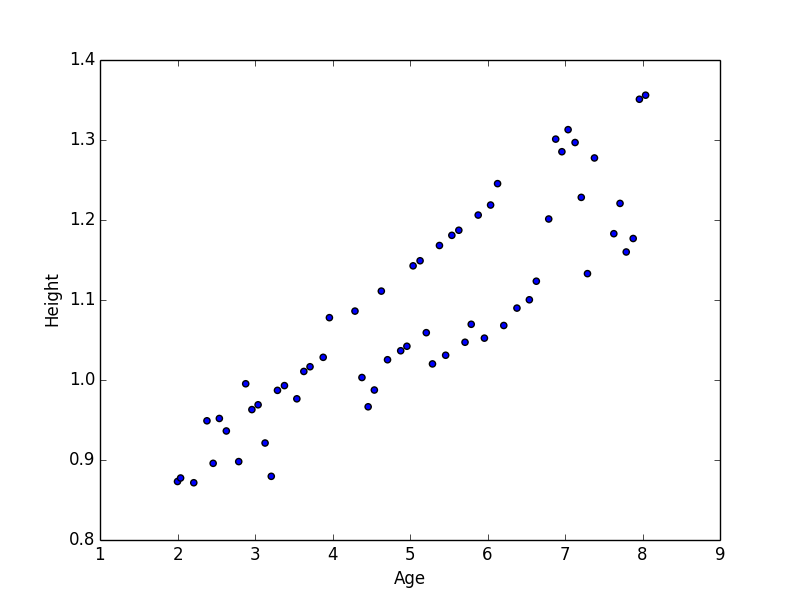
\includegraphics[width=3.0in]{p1_distribution}
    \caption{Training data distribution}
    \label{p1distribution}
\end{figure}

After implementing the Gradient Descent algorithm, I ran it on my test data using $\alpha = 0.05$ and set the number of iterations to 1500. My mean square error was of 0.001825 for the training set. My model was $0.064464x + 0.756075$ as illustrated on Figure \ref{regressionline}. The cost function has a flat bowl shape (see Figure \ref{costfunction}).

\begin{figure}[htb]
\centering
\begin{minipage}{.5\textwidth}
  \centering
  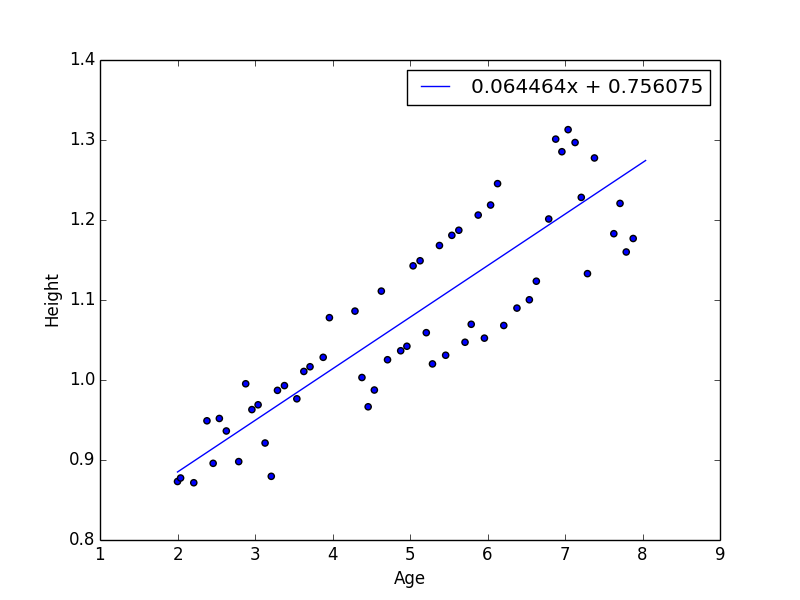
\includegraphics[width=1.0\linewidth]{regression_line}
  \captionof{figure}{Regression line}
  \label{regressionline}
\end{minipage}%
\begin{minipage}{.5\textwidth}
  \centering
  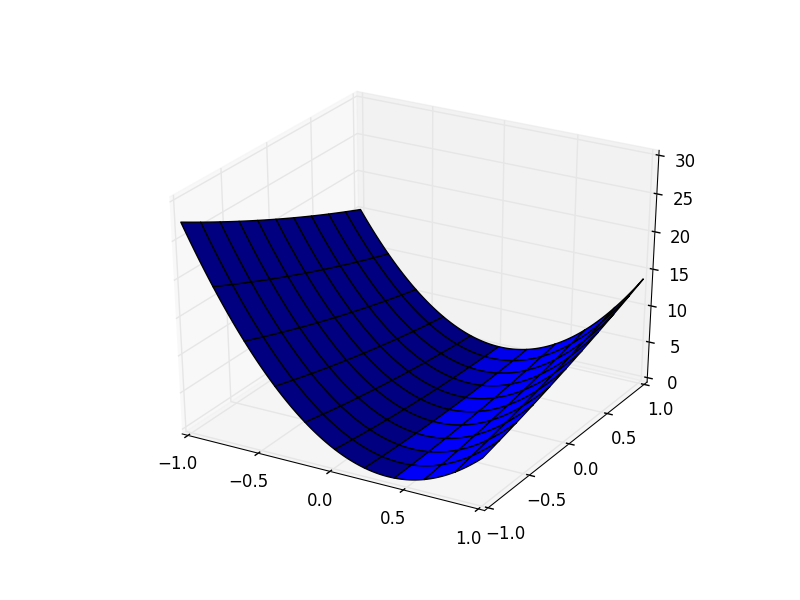
\includegraphics[width=1.0\linewidth]{p1_cost_function}
  \captionof{figure}{Cost function}
  \label{costfunction}
\end{minipage}
\end{figure}


Using my model I predicted that a 4.5 kilos girl would be approximately 1.046164 m tall, which is an accurate estimation. The model also performed well on the test set. The mean square error was 0.003203 for the 20 examples.

\subsection{Linear regression with multiple features}
The second part of this problem consisted in implementing Gradient Descent with multiple features. For this experiment, I used the \path{girls_age_weight_height_2_8.csv} dataset provided.

Before running the Gradient Descent, we were advised to scale the features. Using mean 5.210506 and standard deviaton 1.899482, I scaled the features, getting the desired $\mu(x) = 0$. The next step was choosing the best $\alpha$. I looped through all possible values (0.005, 0.001, 0.05, 0.1, 0.5, 1.0) for the learning rate using number of iterations, applying Gradient Descent for each of them.

\begin{figure}[htb]
    \centering
    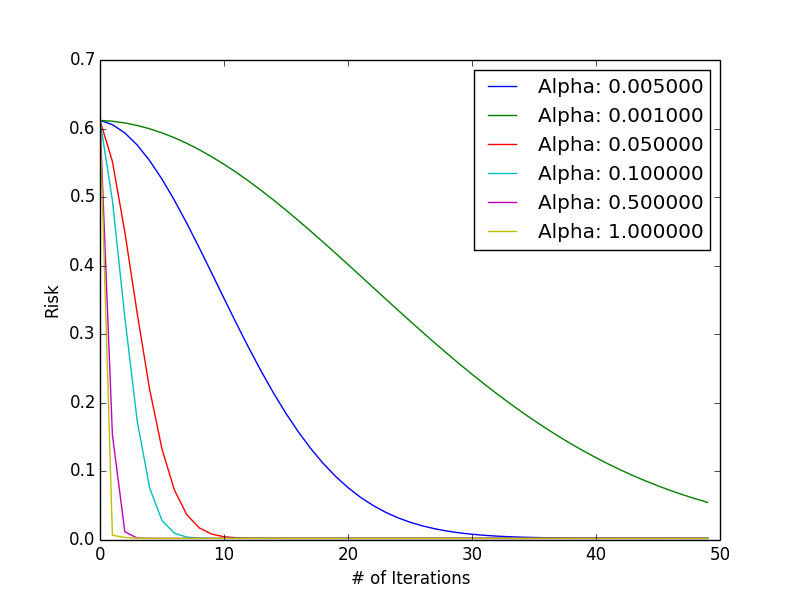
\includegraphics[width=3.0in]{p1_alpha_convergence}
    \caption{Training data distribution}
    \label{costfunction}
\end{figure}

The results for each $\alpha$ is shown on Figure \ref{costfunction}. These results show that smaller values of $\alpha$ tend to converge slower that the larger ones. The best value on this one is 1.0. The $\beta's$ are [1.09646081, 0.12861721, 0.00140248]. A predict height for a 5-year olg girl weighting 20 kilos is 1.082595 m.

\subsubsection{Linear regression with Normal Equations}
Although having the same prediction and the same error, the $\beta's$ aren't the same and that's due to the fact that when I was doing Gradient Descent with multiple variables, I scaled my dataset.

Normal Equations yield the same predictions as Gradient Descent. The reason is that both Normal Equations and Gradient Descent try to minimize the Least Squares. The thing is that NE finds a unique solution that minimizes the least squares. It is not always the best approach because its time complexity is really high. The predicted height for a 5-year olg girl weighting 20 kilos was 1.082595 m.


\section{Problem 2}

On Problem 2 we were asked do perfom classification on a dataset found in \path{chessboard.csv}. First, I trained the data using the three SVM kernels (Linear, Polynomial and RBF). We also needed to train our data using cross-validation with stratified sampling. All of these operations are available out of the box on \path{scikit-learn} package for Python. As extra credit, I also performed classification using other 4 classifiers: K-Nearest Neighbors, Random Forest, ADA Boost and Decision Tree.

\subsection{Training the data}

To train my model I used CVGridSearch from \path{Sklearn} to search for a good set of parameters for each kernel. I perfomed two rounds one using a different number of folds for cross-validation (5 and 10). The C parameter for all SVC was either 1 or 10. For RBC I used $\gamma = {0.1, 1, 10}$. Using a degree below 3 was giving me really poor classification so I decided to cap them from the range. The chosen values for polynomial degree were 4,5 and 6.

The results were pretty solid. Except for the Linear Kernel (which makes sense because the labels can't be separated by a line with this distribution), all of them performed reasonably well. See Figure \ref{main_classifiers} for data distribution and decision boundaries for the SVM classifiers.

\subsection{Results}

I compiled in tables the mean score for each cross-validation run with the possible parameters. The best results for each classifier is colored in green.

\begin{figure}[p]
\centering
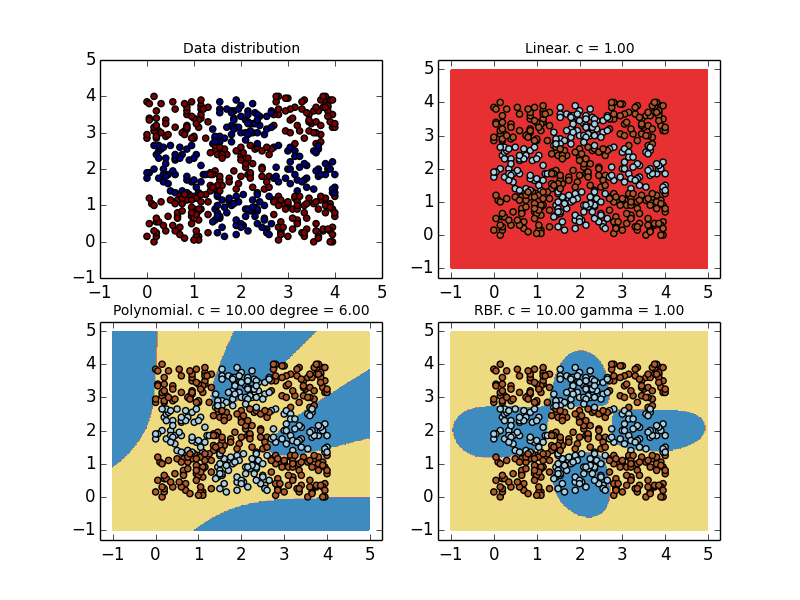
\includegraphics[width=\textwidth]{main_classifiers}
\caption{Data distribution and Decision boundaries for SVM classifiers}
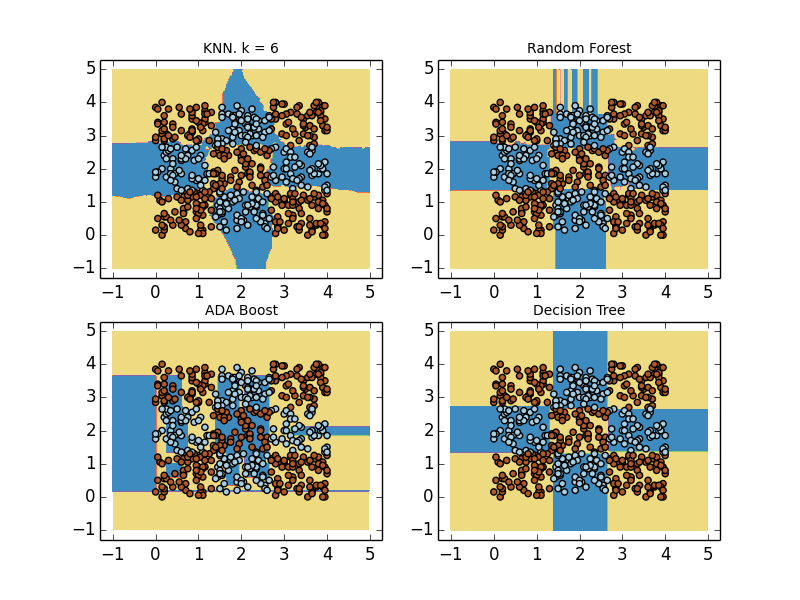
\includegraphics[width=\textwidth]{extra_classifiers}
\caption{Decision boundaries for extra classifiers}
\label{main_classifiers}
\end{figure}

\subsubsection{Linear kernel}

\begin{table}[htb]
\begin{tabular}{|c|c|c|}
\hline
\textbf{K-Folds} & \textbf{C}  & \textbf{Train accuracy}    \\ \hline
\rowcolor[HTML]{34FF34} 
5       & 1  & 0.620000 \\ \hline
5       & 1  & 0.620000 \\ \hline
10      & 10 & 0.620000 \\ \hline
10      & 10 & 0.620000 \\ \hline
\end{tabular}
\end{table}

\subsubsection{Polynomial}

\begin{table}[h]
\begin{tabular}{|c|c|c|c|}
\hline
\textbf{K-folds} & \textbf{C}  & \textbf{Degree} & \textbf{Train accuracy}    \\ \hline
5       & 1  & 4      & 0.706667 \\ \hline
5       & 1  & 5      & 0.733333 \\ \hline
5       & 1  & 6      & 0.730000 \\ \hline
5       & 10 & 4      & 0.713333 \\ \hline
5       & 10 & 5      & 0.726667 \\ \hline
\rowcolor[HTML]{34FF34}
5       & 10 & 6      & 0.736667 \\ \hline
10      & 1  & 4      & 0.710000 \\ \hline
10      & 1  & 5      & 0.730000 \\ \hline
10      & 1  & 6      & 0.730000 \\ \hline
10      & 10 & 4      & 0.716667 \\ \hline
10      & 10 & 5      & 0.730000 \\ \hline
10      & 10 & 6      & 0.733333 \\ \hline
\end{tabular}
\end{table}

\pagebreak

\subsubsection{RBF}

\begin{table}[h]
\begin{tabular}{|c|c|c|c|}
\hline
\textbf{K-Folds} & \textbf{C} & \textbf{Gamma} & \textbf{Train accuracy} \\ \hline
5                & 1          & 0.1            & 0.620000       \\ \hline
5                & 1          & 1              & 0.920000       \\ \hline
5                & 1          & 10             & 0.913333       \\ \hline
5                & 10         & 0.1            & 0.630000       \\ \hline
5                & 10         & 1              & 0.940000       \\ \hline
5                & 10         & 10             & 0.913333       \\ \hline
10               & 1          & 0.1            & 0.620000       \\ \hline
10               & 1          & 1              & 0.926667       \\ \hline
10               & 1          & 10             & 0.930000       \\ \hline
10               & 10         & 0.1            & 0.616667       \\ \hline
\rowcolor[HTML]{34FF34}
10               & 10         & 1              & 0.946667       \\ \hline
10               & 10         & 10             & 0.916667       \\ \hline
\end{tabular}
\end{table}


\subsubsection{K-Nearest Neighbors}

\begin{table}[htb]
\begin{tabular}{|c|c|c|}
\hline
\textbf{K-Fold} & \textbf{N. Neighbors} & \textbf{Train accuracy} \\ \hline
5               & 1           & 0.900000           \\ \hline
5               & 2           & 0.883333           \\ \hline
5               & 3           & 0.916667           \\ \hline
5               & 4           & 0.906667           \\ \hline
5               & 5           & 0.913333           \\ \hline
5               & 6           & 0.923333           \\ \hline
5               & 7           & 0.916667           \\ \hline
5               & 8           & 0.910000           \\ \hline
10              & 1           & 0.910000           \\ \hline
10              & 2           & 0.883333           \\ \hline
10              & 3           & 0.926667           \\ \hline
10              & 4           & 0.930000           \\ \hline
10              & 5           & 0.920000           \\ \hline
\rowcolor[HTML]{34FF34}
10              & 6           & 0.936667           \\ \hline
10              & 7           & 0.930000           \\ \hline
10              & 8           & 0.920000           \\ \hline
\end{tabular}
\end{table}

\pagebreak

\subsubsection{Other classifiers and test scores}

\begin{table}[htb]
\begin{tabular}{|c|c|c|}
\hline
\textbf{Classifier} & \textbf{Train Accuracy} & \textbf{Test Accuracy} \\ \hline
Linear Kernel       & 0.62                    & 0.545000               \\ \hline
Polynomial          & 0.73666666              & 0.700000               \\ \hline
RBF                 & 0.94666666              & 0.955000               \\ \hline
KNN                 & 0.93666666              & 0.945000               \\ \hline
Random Forest       & 1.0                     & 0.945000               \\ \hline
ADA Boost           & 0.743333333333          & 0.605000               \\ \hline
Decision Tree       & 1.0                     & 0.990000               \\ \hline
\end{tabular}
\end{table}

\subsection{Conclusion}

This was a really good exercice for me. I learned tons, not only from the Machine Learning field but how to use Python to produce charts and representations. I also liked the fact that I could found I better predictor than what I initially guessed would be the best (Decision Tree was the best classifier here). Hopefully I would get more hands on experience on this field soon.

\end{document}